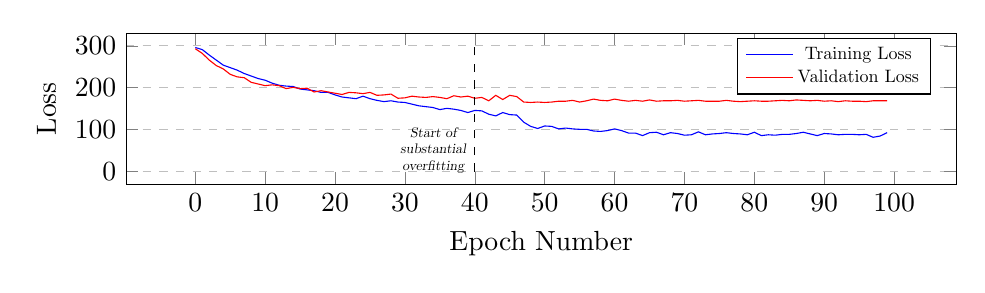
\begin{tikzpicture}
    \begin{axis}[
                height=3.5cm,
                width=\linewidth,
                xlabel={Epoch Number},
                ylabel={Loss},
                legend pos=north east,
                ymajorgrids=true,
                grid style=dashed,
                legend style={nodes={scale=0.65, transform shape}},
            ]
        %
        % TRAINING LOSS
        %
        \addplot[color=blue] coordinates {
            (0, 296) (1, 291) (2, 278) (3, 266) (4, 254) (5, 248) (6, 242) (7,
            234) (8, 228) (9, 222) (10, 218) (11, 211) (12, 206) (13, 204) (14,
            203) (15, 197) (16, 195) (17, 193) (18, 189) (19, 189) (20, 183)
            (21, 178) (22, 176) (23, 174) (24, 180) (25, 174) (26, 170) (27,
            167) (28, 169) (29, 166) (30, 165) (31, 161) (32, 157) (33, 155)
            (34, 153) (35, 148) (36, 151) (37, 149) (38, 146) (39, 141) (40,
            146) (41, 145) (42, 137) (43, 133) (44, 141) (45, 136) (46, 135)
            (47, 118) (48, 108) (49, 103) (50, 109) (51, 108) (52, 102) (53,
            104) (54, 102) (55, 101) (56, 101) (57, 97) (58, 96) (59, 98) (60,
            102) (61, 98) (62, 92) (63, 92) (64, 86) (65, 93) (66, 94) (67, 88)
            (68, 93) (69, 91) (70, 87) (71, 88) (72, 95) (73, 88) (74, 90) (75,
            91) (76, 93) (77, 91) (78, 90) (79, 88) (80, 94) (81, 86) (82, 88)
            (83, 87) (84, 89) (85, 89) (86, 91) (87, 94) (88, 90) (89, 86) (90,
            91) (91, 90) (92, 88) (93, 89) (94, 89) (95, 88) (96, 89) (97, 82)
            (98, 85) (99, 93)
        };
        \addlegendentry{Training Loss}
        %
        % VALIDATION LOSS
        %
        \addplot[color=red] coordinates {
            (0, 293) (1, 282) (2, 266) (3, 253) (4, 245) (5, 232) (6, 226) (7,
            224) (8, 213) (9, 209) (10, 205) (11, 207) (12, 205) (13, 198) (14,
            201) (15, 198) (16, 199) (17, 190) (18, 193) (19, 190) (20, 187)
            (21, 184) (22, 189) (23, 188) (24, 186) (25, 189) (26, 182) (27,
            183) (28, 185) (29, 175) (30, 176) (31, 180) (32, 178) (33, 177)
            (34, 179) (35, 177) (36, 174) (37, 181) (38, 178) (39, 180) (40,
            175) (41, 177) (42, 169) (43, 182) (44, 172) (45, 182) (46, 179)
            (47, 166) (48, 165) (49, 166) (50, 165) (51, 166) (52, 168) (53,
            168) (54, 170) (55, 166) (56, 169) (57, 173) (58, 170) (59, 169)
            (60, 173) (61, 170) (62, 168) (63, 170) (64, 168) (65, 171) (66,
            168) (67, 169) (68, 169) (69, 170) (70, 168) (71, 169) (72, 170)
            (73, 168) (74, 168) (75, 168) (76, 170) (77, 168) (78, 167) (79,
            168) (80, 169) (81, 168) (82, 168) (83, 169) (84, 170) (85, 169)
            (86, 171) (87, 170) (88, 169) (89, 170) (90, 168) (91, 169) (92,
            167) (93, 169) (94, 168) (95, 168) (96, 167) (97, 169) (98, 169)
            (99, 169)
        };
        %
        % OVERFITTING LINE
        %
        \addplot[mark=none, dashed] coordinates {(40, 0) (40, 300)}
            node[midway, scale=0.5, yshift=-3em, xshift=-3em] {
                \parbox{5em}{\slshape\centering%
                    Start of substantial overfitting}
            };
        \addlegendentry{Validation Loss}
    \end{axis}
\end{tikzpicture}

